Hvis der indgår et teoretisk problem: Omfatter hovedteksten et teori-afsnit?\\
\section{Indlening til hovedafsnit}
Indeholder indledningen en overordnet introduktion til afsnittet?\\
\section{Første elaborationsfasen}
\subsection{Indledning til første elaborationsfasen}
Formålet med elaborationsfasen er at skabe en interaktiv udvikling af produktet MMMI´s\footnote{{mangfoldig manager management instruments}} funktionalitet. Denne udvikling sker på baggrund af inceptionsfasen\footnote{{Bilag : Inceptionss dokumentet}}, hvor der blev opstillet en række krav til MMMI-projektet.  For at kunne nå de mål bliver der lagt lavet nogle mindre iterationer her under krav, analyse, design, kode og test som arbejdes med ud fra de overordnede kravspecifikationer. Målet er at får en funktionel kode færdig til elaborationsmilepælen. 



\section{Overordnet kravspecifikation (resume, opdateret)}
Indeholder afsnittet et opdateret resumé  af systemafgrænsningen fra inceptionsdokumentet.
\section{Detaljeret kravspecifikation}
Omfatter den detaljerede kravspecifikation\\
Detaljeret brugsmønsterdiagram (hvis relevant)\\
Detaljerede brugsmønsterbeskrivelser\\
Detaljerede beskrivelser af supplerende krav Fx organiseret efter FURPS+\\
\section{Analyse}
Omfatter afsnittet overvejelser, beslutninger og resultater vedr.\\
Den statiske side af analysemodel\\
Den dynamiske side af analysemodel\\
\section{Design}
Omfatter afsnittet overvejelser, beslutninger og resultater vedr.\\
Softwarearkitektur\\
Subsystemdesign\\
Den statiske side af designmodel\\
Den dynamiske side af designmodel\\
Design af persistens\\
Databasedesign\\
\section{Implementering}
Omfatter afsnittet overvejelser, beslutninger og resultater vedr.\\  konvertering fra design til kode illustreret gennem udvalgte centrale eksempler, samt andre vigtige implementeringsbeslutninger
Omfatter afsnittet implementering af database.


\begin{figure}
\begin{lstlisting}]
/**
     *
     * @param searchWord
     * @return
     */
    public List<Case> search(String searchWord) {

        List<Case> listCases = new ArrayList<>();

        for (Case searchCase : caseMap.values()) {
            if (searchCase.getRegardingCitizen().getCprNumber().equalsIgnoreCase(searchWord)
                    || searchCase.getCaseNumber().equalsIgnoreCase(String.valueOf(searchWord))
                    || searchCase.getRegardingCitizen().getName().equalsIgnoreCase(searchWord)) {
                listCases.add(searchCase);
            }
        }

        return listCases;
    }


\end{lstlisting}
\caption{kode : seartch}
\label{kode:Search}
\end{figure}



\begin{figure}
  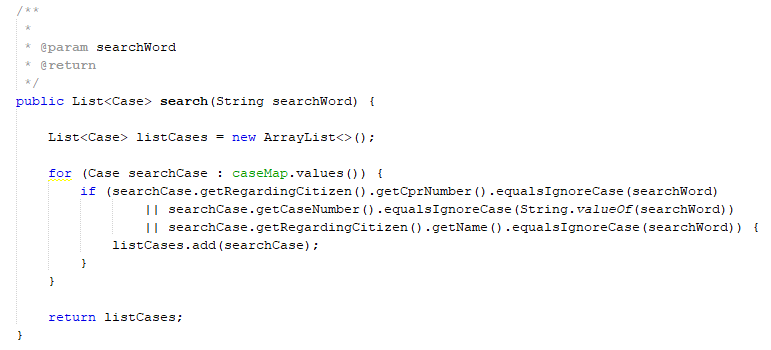
\includegraphics[width=\linewidth]{./PNG/code_search.PNG} 
  \caption{Kode: search}
  \label{kode:Search}
\end{figure}


\section{Test}
Omfatter afsnittet en beskrivelse af de udførte test samt resultatet af dem.\\
Er der medtaget resultater både fra iteration 1 og fra iteration 2?\\
